\subsubsection{Smartphone als Master}
	Ein Smartphone vereint mehrere für die Realisation des Produkts benötigte 
	Komponenten (Kamera, drahtlose Schnittstelle, Recheneinheit, Endsignalausgabe) 
	in einem Gerät. Des Weiteren sind heutige Smartphones verhältnismässig 
	leistungsfähig, die Berechnungen für die Objekterkennung können direkt auf 
	dem Gerät erfolgen und durch den USB-Port wird eine sichere Verbindung zum 
	Controller gewährleistet. Die Alternative, einzelne Module (Kamera, drahtlose 
	Schnittstelle, Recheneinheit) zu verbauen, gewährleistet eine erhöhte 
	Flexibilität, allerdings verbunden mit steigendem Aufwand und höherem Preis. 
	Zudem hätte die Verwendung von Einzelmodulen unter Umständen eine 
	Gewichtszunahme zur Folge, da keine vergleichbare Kompaktheit wie bei einem 
	Smartphone besteht. Der Einsatz eines Smartphones bietet im Vergleich zu 
	einzelnen Modulen somit entscheidende Vorteile.\\
	\\
	Es ist wichtig, dass die Kamera das Spielfeld komplett erfassen kann, 
	weswegen das Smartphone vorne am Gerät angebracht wird. Eine Befestigung 
	an der Front des Gerätes bietet sich an, da dort eine hohe Stabilität 
	vorhanden ist, was für eine optimale Bildaufnahme wichtig ist.\\
	\\
	Falls die Korberkennung nicht auf dem Smartphone umgesetzt werden kann, 
	wird die Berechnung auf einem externen PC durchgeführt. In diesem Fall wird 
	eine Webcam am PC angeschlossen. Die Montage an der Abwurfeinheit bliebe unverändert. Genauso die Kommunikation mit dem Controller, welche immer noch mittels USB realisiert würde.
	%
	\newpage
	\paragraph{Korberkennung}$~~$\vspace{2mm}\\
		Für die Bestimmung der Position des Korbes wurde ein Algorithmus 
		eigens entwickelt und in Java implementiert. Auf die Verwendung eines 
		Frameworks (wie beispielsweise OpenCV) wurde verzichtet. Grund dafür 
		liegt in der statischen Problemstellung: Hintergrund, Korbform und -farbe 
		sind immer gleich, was die Problemstellung stark vereinfacht und die Verwendung eines komplexeren Algorithmus hinfällig macht. Somit kann die Erkennungsmechanik einfach und statisch gehalten werden. Unterstützt wird diese Entscheidung auch durch den grösseren Lerneffekt, welche eine Eigenproduktion mit sich bringt. \\
		\\
		Der Algorithmus 
		basiert auf der Tatsache, dass der Korb deutlich dunkler als der 
		Hintergrund ist. Damit mit einem aufgenommenen Bild gearbeitet werden kann, 
		müssen die Ränder abgeschnitten werden. Dies ist notwendig, da die Kamera einen 
		grossen horizontalen Öffnungswinkel aufweist. Dementsprechend geht der 
		Bildbereich links und rechts deutlich über das Spielfeld 
		hinaus, was das Resultat verfälschen könnte. Als zweiter Schritt wird 
		über sämtliche Pixel des Bildes iteriert. Dabei wird für jedes Pixel die 
		Helligkeit anhand einer vordefinierten Schwelle bestimmt, ob es zum 
		Hintergrund (heller) oder zum Korb (dunkel) gehört. Zur Bestimmung der Helligkeit eines Pixels anhand eines RGB Wertes gibt es mehrere Möglichkeiten, welche sich in Genauigkeit und Performance unterscheiden \cite{S:RGB}. Ein genügend hoher 
		Kontrast ist an dieser Stelle entscheidend. Vor allem Schattenwürfe durch 
		seitliche Beleuchtung stellen ein Problem dar. Deshalb wurde diesbezüglich 
		ein erster Test des entwickelten Prototypen mit zwei Scheinwerfern 
		durchgeführt (siehe Kapitel \ref{chap:LichtTest}). Als nächster Schritt 
		wird der Schwerpunkt der dunklen Pixel bestimmt und anhand des gefundenen 
		Schwerpunktes entweder von links oder von rechts her in einem bestimmten 
		horizontalen Bereich (der Korb befindet sich immer auf der selben Höhe)
		über die Pixel iteriert um dabei eine feste Kontur zu finden. Diese feste 
		Kontur wird dabei definiert durch eine bestimmte Anzahl weisse Pixel, auf 
		welche wiederum eine Menge schwarzer Pixel folgen muss. Da dieser Prozess 
		immer in derselben horizontalen Ebene stattfindet kann durch eine 
		abschliessende Berechnung der Mittelpunkt des Korbes und der damit 
		verbundene Winkel des Ballwerfers zum Korb trigonometrisch bestimmt werden.
		Der Ablauf ist in der Abbildung \ref{fig:KorberkennungFlowchart} grafisch 
		dargestellt.
		\begin{figure}[h!]
			\centering
			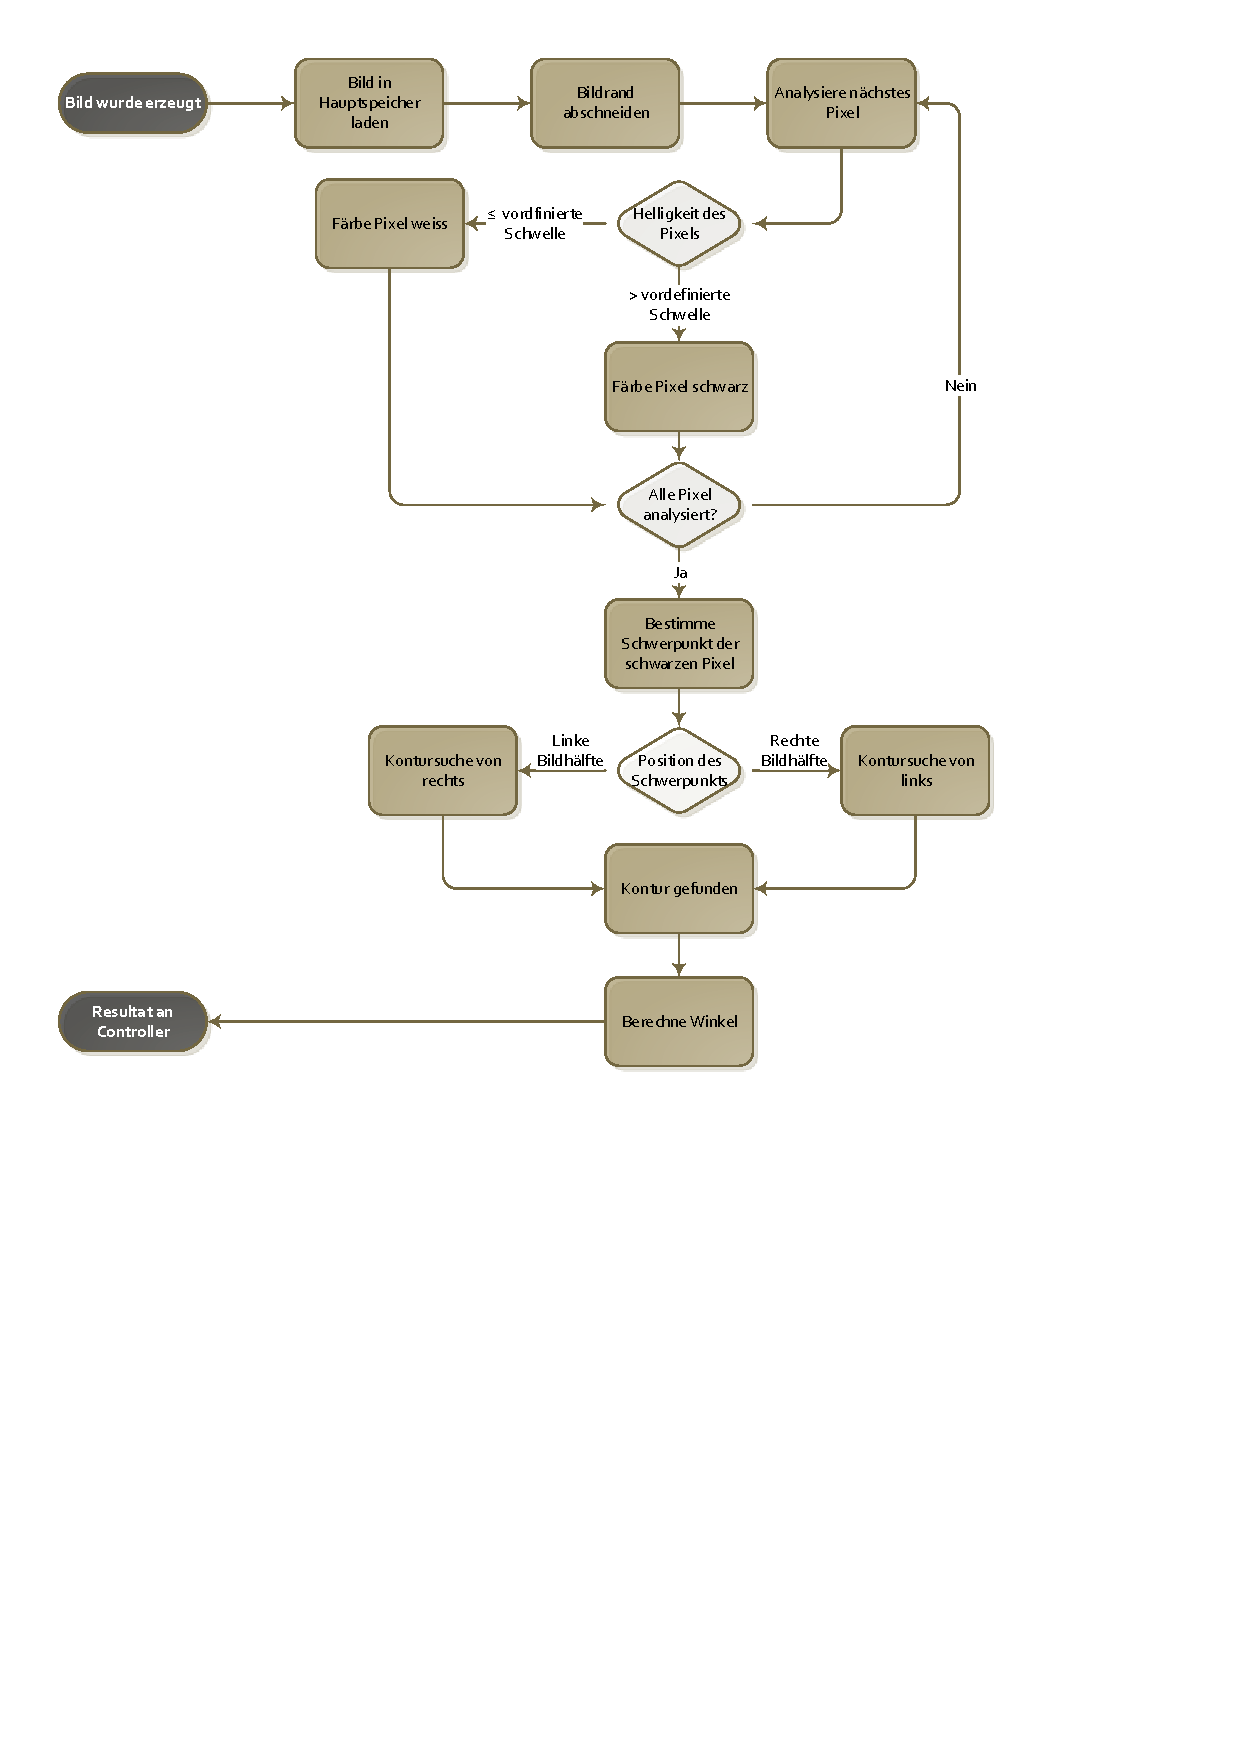
\includegraphics[width=1\textwidth,clip,trim=9mm 115mm 41mm 9mm]
			{Enddokumentation/Loesungskonzept/Bilder/Flowchart_Korberkennung.pdf}
			\caption{Ablaufdiagramm zum Korberkennungs-Algorithmus}
			\label{fig:KorberkennungFlowchart}
		\end{figure}